\documentclass[a4paper,11pt]{ctexart}

\usepackage[top=1.8cm,bottom=1.8cm,left=2.1cm,right=2.1cm]{geometry}
\usepackage{amsmath,amssymb}
\usepackage{graphicx}
\usepackage{enumitem}
\usepackage{fancyhdr}
\usepackage{lastpage}

\pagestyle{fancy}
\fancyhf{}
\renewcommand{\headrulewidth}{0pt}
\fancyfoot[C]{\small 第~\thepage~页\quad 共~\pageref{LastPage}~页}

\linespread{1.28}
\setlength{\parindent}{0pt}

\newcommand{\dd}{\,\mathrm{d}}
\newcommand{\e}{\mathrm{e}}
\newcommand{\blank}[1][2.2cm]{\underline{\hspace{#1}}}
\newcommand{\score}[1]{\hfill{\text{（#1 分）}}}

\begin{document}

\begin{center}
  {\Large\bfseries 2020～2021 学年第一学期}\\[0.5em]
  {\Large\bfseries 《微积分（一）》课程考试试卷（A 卷）解答}
\end{center}

\vspace{0.6em}

\textbf{一、单项选择题（每小题 4 分，4 个小题共 16 分，将结果写在答题卡上。）}

\begin{enumerate}[label=\arabic*., leftmargin=2em, itemsep=0.7em, topsep=0.6em]
  \item 曲线 $y=(x-1)(x-2)(x-3)$ 与 $x$ 轴所围成的图形的面积可表示为 \textbf{【C】}。

  A. $\displaystyle\int_1^3 (x-1)(x-2)(x-3)\dd x$

  B. $-\displaystyle\int_1^3 (x-1)(x-2)(x-3)\dd x$

  C. $\displaystyle\int_1^2 (x-1)(x-2)(x-3)\dd x - \int_2^3 (x-1)(x-2)(x-3)\dd x$

  D. $\displaystyle\int_2^3 (x-1)(x-2)(x-3)\dd x - \int_1^2 (x-1)(x-2)(x-3)\dd x$

  \item 设 $f(x)$ 是周期为 $T$ 的连续函数，$a$ 为常数，则下列必为周期函数的是 \textbf{【A】}。

  A. $\displaystyle\int_x^{x+a} f(t)\dd t$ \qquad\quad
  B. $\displaystyle\int_a^{x+T} f(t)\dd t$ \qquad\quad
  C. $\displaystyle\int_a^x f(t+T)\dd t$ \qquad\quad
  D. $\displaystyle\int_a^x f(t)\dd t$

  \item 已知函数 $f(x)=\begin{cases}2(x-1), & x<1,\\ \ln x, & x\ge 1,\end{cases}$ 则 $f(x)$ 的一个原函数是 \textbf{【D】}。

  \makebox[0.48\linewidth][l]{A. $F(x)=\begin{cases}(x-1)^2, & x<1,\\ x(\ln x-1), & x\ge 1.\end{cases}$}B. $F(x)=\begin{cases}(x-1)^2, & x<1,\\ x(\ln x+1)-1, & x\ge 1.\end{cases}$

  \vspace{0.4em}
  \makebox[0.48\linewidth][l]{C. $F(x)=\begin{cases}(x-1)^2, & x<1,\\ x(\ln x+1)+1, & x\ge 1.\end{cases}$}D. $F(x)=\begin{cases}(x-1)^2, & x<1,\\ x(\ln x-1)+1, & x\ge 1.\end{cases}$

  \item 设 $I_1=\displaystyle\int_2^1 \e^x\dd x$，$I_2=\displaystyle\int_2^1 \e^{x^2}\dd x$，$I_3=\displaystyle\int_2^1 (1+x)\dd x$，则 \textbf{【B】}。

  A. $I_1>I_2>I_3$ \qquad\quad
  B. $I_3>I_1>I_2$ \qquad\quad
  C. $I_1>I_3>I_2$ \qquad\quad
  D. $I_2>I_1>I_3$
\end{enumerate}

\vspace{0.8em}

\textbf{二、填空题（每小题 5 分，4 个小题共 20 分，将计算结果写在答题卡上。）}

\begin{enumerate}[label=\arabic*., start=5, leftmargin=2em, itemsep=0.8em, topsep=0.5em]
  \item $\displaystyle\int_{-\frac{\pi}{2}}^{\frac{\pi}{2}}\left(\frac{\sin x}{1+\cos x}+|x|\right)\dd x=\underline{\ \pi^2/4\ }$。

  \textbf{解}：$\displaystyle\int_{-\frac{\pi}{2}}^{\frac{\pi}{2}}\left(\frac{\sin x}{1+\cos x}+|x|\right)\dd x = 2\int_0^{\frac{\pi}{2}}x\dd x = \frac{\pi^2}{4}$。

  \item $\displaystyle\int_0^1 x(1-x)^{99}\dd x=\underline{\ 1/10100\ }$。

  \textbf{解}：令 $t=1-x$，则 $\displaystyle\int_0^1 x(1-x)^{99}\dd x = \int_0^1 t^{99}(1-t)\dd t = \frac{1}{100}-\frac{1}{101} = \frac{1}{10100}$。

  \item 设 $f(x)$ 的一个原函数是 $x\ln x$，则 $\displaystyle\int xf'(x)\dd x=\underline{\ x+C\ }$。

  \textbf{解}：$f(x)=(x\ln x)'=\ln x+1$，$f'(x)=\dfrac{1}{x}$，故 $\displaystyle\int xf'(x)\dd x=x+C$。

  \item $\displaystyle\int_1^3 \frac{1}{\sqrt{x}(1+x)}\dd x=\underline{\ \pi/6\ }$。

  \textbf{解}：$\displaystyle\int_1^3\frac{1}{\sqrt{x}(1+x)}\dd x = 2\int_1^3\frac{1}{1+x}\dd\sqrt{x} = \left.2\arctan\sqrt{x}\right|_1^3 = \frac{\pi}{6}$。
\end{enumerate}

\vspace{0.8em}

\textbf{三、计算题（每小题 8 分，4 个小题共 32 分，必须写出主要计算过程。）}

\begin{enumerate}[label=\arabic*., start=9, leftmargin=2em, itemsep=0.9em, topsep=0.5em]
  \item 求极限 $l=\displaystyle\lim_{n\to\infty}\ln\sqrt[n]{\left(1+\frac{1}{n}\right)^2\left(1+\frac{2}{n}\right)^2\cdots\left(1+\frac{n}{n}\right)^2}$。

  \textbf{解}：
  \begin{align*}
    l &= \lim_{n\to\infty}\sum_{i=1}^n \frac{2}{n}\ln\left(1+\frac{i}{n}\right) \tag*{（3 分）}\\
      &= 2\int_0^1\ln(1+x)\dd x \tag*{（6 分）}\\
      &= 4\ln 2 - 2. \tag*{（8 分）}
  \end{align*}

  \item 计算 $l=\displaystyle\lim_{x\to 0}\frac{\displaystyle\int_0^x t\ln(1+t\sin t)\dd t}{1-\cos x^2}$。

  \textbf{解}：
  \begin{align*}
    l &= \lim_{x\to 0}\frac{x\ln(1+x\sin x)}{2x\cdot\sin x^2} \tag*{（4 分）}\\
      &= \lim_{x\to 0}\frac{x\cdot x\sin x}{2x^3} \tag*{（6 分）}\\
      &= \frac{1}{2}. \tag*{（8 分）}
  \end{align*}

  \item 计算 $I=\displaystyle\int_0^{\ln 5}\frac{\e^x\sqrt{\e^x-1}}{\e^x+3}\dd x$。

  \textbf{解}：令 $t=\sqrt{\e^x-1}$，则 $x=\ln(1+t^2)$，$\dd x=\dfrac{2t}{1+t^2}\dd t$，\score{3}
  \begin{align*}
    I &= \int_0^2\frac{(t^2+1)t}{t^2+4}\cdot\frac{2t}{t^2+1}\dd t
       = 2\int_0^2\frac{t^2}{t^2+4}\dd t
       = 2\int_0^2\left(1-\frac{4}{t^2+4}\right)\dd t \tag*{（6 分）}\\
      &= \left[2t - 4\arctan\frac{t}{2}\right]_0^2 = 4 - \pi. \tag*{（8 分）}
  \end{align*}

  \item 求 $I=\displaystyle\int_0^{+\infty}\frac{\ln(1+x)}{(1+x)^2}\dd x$。

  \textbf{解}：
  \begin{align*}
    I &= -\int_0^{+\infty}\ln(1+x)\dd\frac{1}{1+x} \tag*{（3 分）}\\
      &= -\left[\left.\frac{\ln(1+x)}{1+x}\right|_0^{+\infty} - \int_0^{+\infty}\frac{1}{(1+x)^2}\dd x\right] \\
      &= \int_0^{+\infty}\frac{1}{(1+x)^2}\dd x \tag*{（6 分）}\\
      &= 1. \tag*{（8 分）}
  \end{align*}
\end{enumerate}

\vspace{0.8em}

\textbf{四、应用题（每小题 8 分，2 个小题共 16 分，必须写出主要过程。）}

\begin{enumerate}[label=\arabic*., start=13, leftmargin=2em, itemsep=1.0em, topsep=0.5em]
  \item 计算抛物线 $y^2=4(x+1)$ 与 $y^2=4(1-x)$ 所围成的平面图形的面积。

  \textbf{解}：
  \begin{minipage}[t]{0.60\linewidth}
    \begin{align*}
      A &= \int_{-2}^2\left[\left(1-\frac{y^2}{4}\right)-\left(\frac{y^2}{4}-1\right)\right]\dd y \tag*{（4 分）}\\
        &= 2\int_{-2}^2\left(1-\frac{y^2}{4}\right)\dd y \\
        &= 4\int_0^2\left(1-\frac{y^2}{4}\right)\dd y = \frac{16}{3}. \tag*{（8 分）}
    \end{align*}
  \end{minipage}
  \hfill
  \begin{minipage}[t]{0.36\linewidth}
    \vspace{0pt}
    \centering
    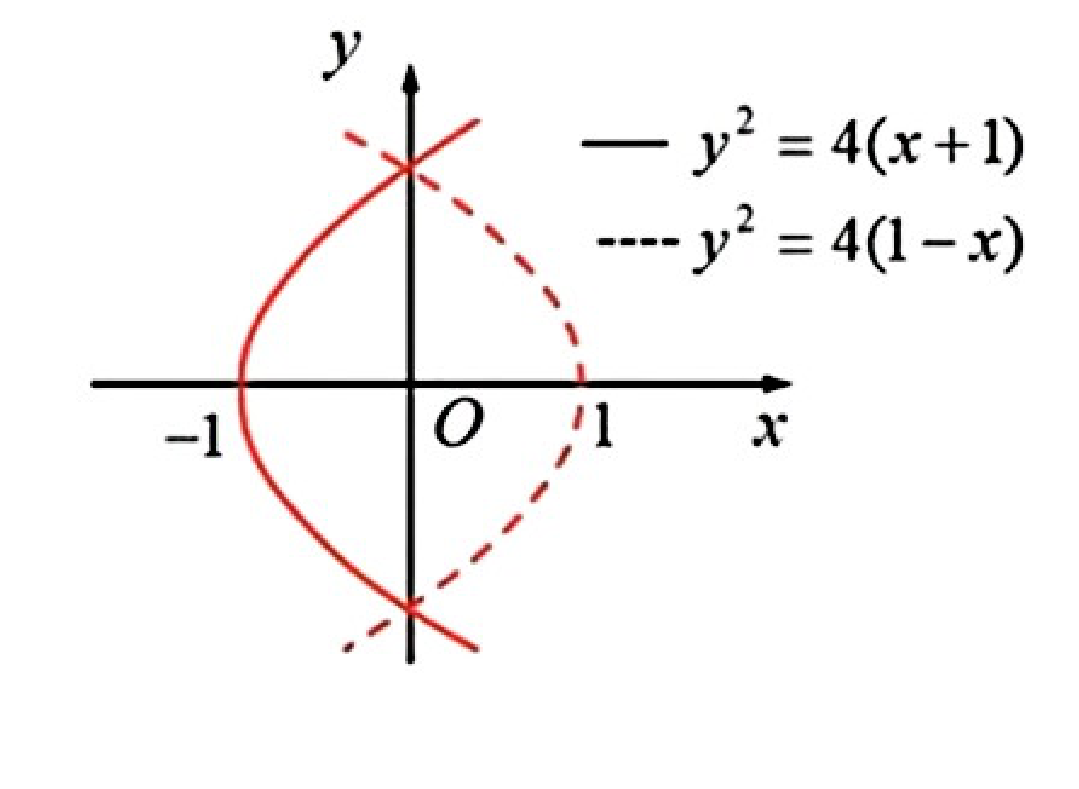
\includegraphics[width=0.95\linewidth]{assets_文字版/20-21答案_q13_fig.png}
  \end{minipage}

  \item 设 $D$ 是由 $y=(x-1)^2$、$x$ 轴、$y$ 轴以及 $x=2$ 所围成的平面区域，求 $D$ 绕 $y$ 轴旋转一周所得的旋转体体积。

  \textbf{解}：取 $x$ 为积分变量，$x\in[0,2]$，

  \begin{minipage}[t]{0.60\linewidth}
    \begin{align*}
      V &= 2\pi\int_0^2 x(x-1)^2\dd x \tag*{（4 分）}\\
        &= 2\pi\int_0^2(x^3-2x^2+x)\dd x \\
        &= \frac{4}{3}\pi. \tag*{（8 分）}
    \end{align*}
  \end{minipage}
  \hfill
  \begin{minipage}[t]{0.36\linewidth}
    \vspace{0pt}
    \centering
    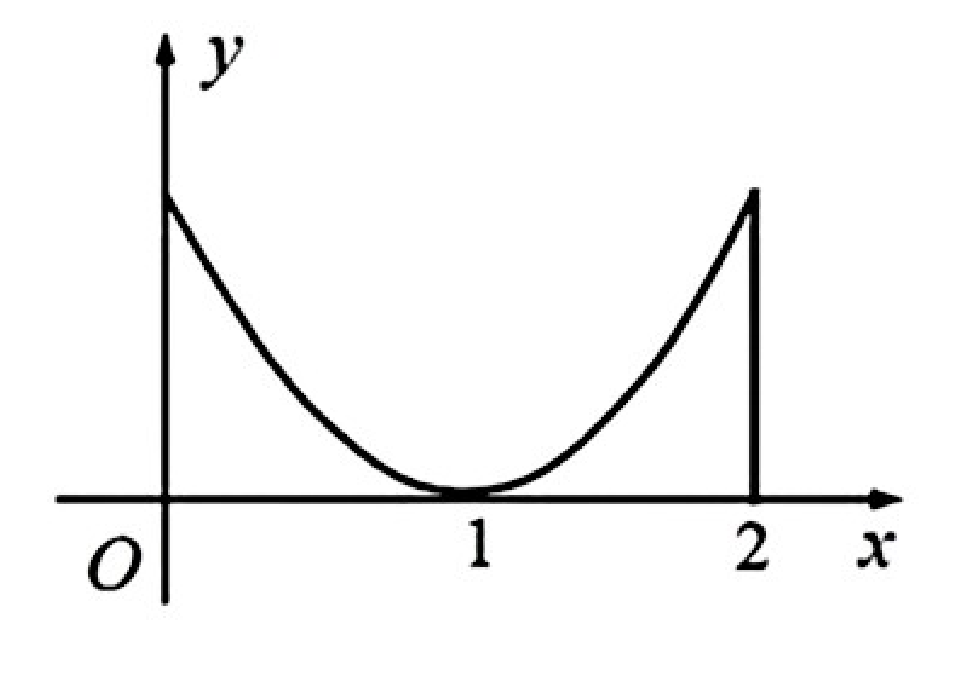
\includegraphics[width=0.95\linewidth]{assets_文字版/20-21答案_q14_fig.png}
  \end{minipage}
\end{enumerate}

\vspace{0.8em}

\textbf{五、综合题（每小题 8 分，2 个小题共 16 分，必须写出主要过程。）}

\begin{enumerate}[label=\arabic*., start=15, leftmargin=2em, itemsep=0.9em, topsep=0.5em]
  \item 设 $f(x)$ 在 $\left[0,\dfrac{\pi}{2}\right]$ 上连续，且满足 $f(x)=\cos x+\displaystyle\int_0^{\frac{\pi}{2}}f(t)\dd t$，求 $f(x)$。

  \textbf{解}：设 $A=\displaystyle\int_0^{\frac{\pi}{2}}f(t)\dd t$，则 $f(x)=\cos x+A$，\score{3}

  方程两边在 $\left[0,\dfrac{\pi}{2}\right]$ 上对 $x$ 积分，得
  \[
    A=\int_0^{\frac{\pi}{2}}\cos x\dd x + A\int_0^{\frac{\pi}{2}}\dd x = 1+\frac{\pi}{2}A \tag*{（6 分）}
  \]
  解出 $A=\dfrac{2}{2-\pi}$，所以 $f(x)=\cos x+\dfrac{2}{2-\pi}$。\score{8}

  \item 设函数 $f(x)$ 在 $[a,b]$ 上连续，$f(x)>0$，又 $F(x)=\displaystyle\int_a^x f(t)\dd t+\int_b^x\frac{1}{f(t)}\dd t$，试证：$F(x)=0$ 在 $[a,b]$ 中有且仅有一个实根。

  \textbf{证}：由题设知 $F(x)$ 在 $[a,b]$ 上连续，且 $F(a)=\displaystyle\int_b^a\frac{1}{f(t)}\dd t<0$，$F(b)=\displaystyle\int_a^b f(t)\dd t>0$。

  根据零点定理知 $F(x)=0$ 在 $[a,b]$ 中有实根，\score{4}

  又 $F'(x)=\left(\displaystyle\int_a^x f(t)\dd t+\int_b^x\frac{1}{f(t)}\dd t\right)'=f(x)+\dfrac{1}{f(x)}\ge 2$，

  即 $F(x)$ 在 $[a,b]$ 上严格单调递增，\score{6}

  故 $F(x)=0$ 在 $[a,b]$ 中有且仅有一个实根。\score{8}
\end{enumerate}

\end{document}
